


We are seeking numerical methods which, when synthesized and simulated on a quantum device, undergo a speedup relative to the original design implemented on a standard electronic computer. To this end we have discussed several potential methods that could take advantage of the design of a quantum computer. they are listed in a table below: 

[INSERT TABLE HERE]

We also plan to take advantage of previous work in the realm of quantum summation and integration [cite papers]. Although we will make use of these quantum algorithms in our research, the real utility of this project is seen in the next section where previous work by the authors will be discussed. 

The problem itself is extremely practical as we are entering the age of big data, where these numerical methods need to be implemented in more efficient ways to balance increasing data set sizes. While the scope of this project is rather large, it will become obvious in the next section why this is a feasible year-long project. 

While we believe that there is a potentially large class of algorithms from traditional numerical methods that will undergo a speedup when synthesized for quantum computers we are not limiting ourselves there, we will also attempt to find statistical procedures (such as hypothesis testing) that could undergo speedup on quantum machines. 
    %\begin{figure} [h!]
      %  \centering
     %   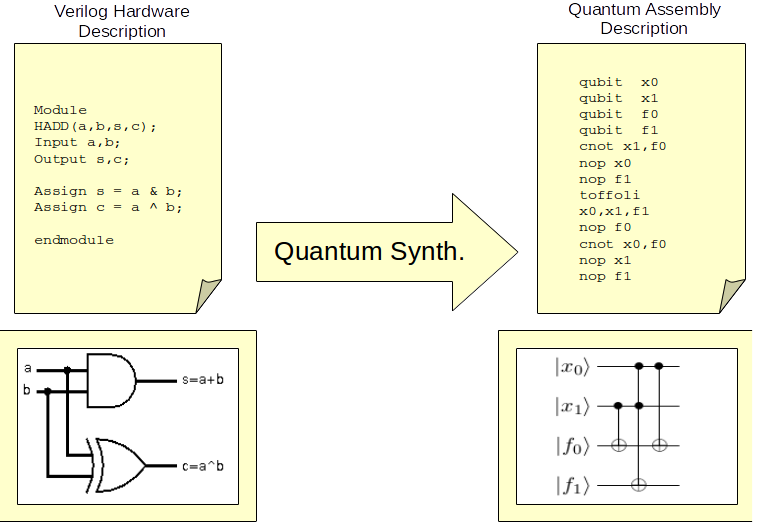
\includegraphics[scale = 0.35]{QuantumSynthesis.png}
    %\end{figure}

